\subsection{Expectimax}
\lezione{Lezione 10}{31/10/2024}
Finora i giochi considerati sono stati deterministici: a partire dall'assunzione di razionalità dell'agente avversario era 
facile prevedere la mossa scelta da costui nell'albero di gioco, per cui era possibile sempre massimizzare il valore di MINIMAX.
Il discorso cambia quando entra in gioco una variabile aleatoria che rende \textbf{stocastica} la natura del gioco. Per modellare
questo tipo di giochi, si introduce un nuovo giocatore detto \textit{Nature} $\mathcal{N}$ che ha le seguenti caratteristiche:
\begin{itemize}
    \item Tutti i player conoscono la strategia di $\mathcal{N}$
    \item La strategia di $\mathcal{N}$ è mista e la sua distribuzione $\Pi$ di probabilità è nota
    \item $\mathcal{N}$ non riceve \textit{payoff}
\end{itemize}
Dal momento che non si sa apriori l'esito delle mosse di $\mathcal{N}$, l'algoritmo può solo massimizzare il \textbf{Valore Atteso}
dello stato; per questo motivo l'algoritmo MINIMAX dei giochi Stocastici è detto \textbf{EXPECTIMAX}.
Anche in questo caso possiamo implementare \textbf{pruning} questa volta basati su bound di valore atteso dei nodi.

\subsubsection{Monte Carlo Tree Search (MTSC)}
Sebbene si possa pensare che l'incertezza e stimare troppo possano creare troppi ostacoli, in realtà questa volta non è cosi:
se il modello probabilistico su cui si basa la stima è corretta, e se la stima è non deviata e consistente, alla lunga la stima
tenderà al valore effettivo di MINIMAX del nodo.
Su questo principio si basa il \textbf{Monte Carlo Tree Search}: quest'algoritmo, oltre a selezionare ed espandere un nodo, introduce
una fase di \textbf{simulazione}, ossia gioca, a partire da un determinato stato, milioni di partite (giocate a caso) per "raffinare" sempre di più la stima 
del valore atteso di una particolare azione tra quelle disponibili

\subsubsection{Multi-Armed Bandit Problem (MAB)}
Chiaramente ci aspettiamo che il MTSC scelga una mossa in un tempo finito, per cui il numero di simulazioni che potrà effettuare
per le varie azioni possibili sarà limitato. Sarà necessario quindi distribuire questa risorsa tra le varie azioni
in modo da non escludere alcuna possibilità e dunque perdere l'ottimalità. 
\paragraph{Approccio Naive.}Si potrebbe scegliere di equidistribuire le simulazioni a tutte le azioni, pure a quelle
meno promettenti. In questo modo, alla fine, si sceglie la mossa $a^* = \arg \max_i \{\omega_i\}$.\\

Quest'approccio funziona, ma si può fare di meglio: quando devo esplorare tutte le azioni? Quando scommetto di più sull'azione
migliore? Questo viene detto \textbf{Dilemma Exploration/Exploitation} e possiamo formularlo con il problema \textbf{Multi-Armed Bandit Problem} che recita cosi:
\begin{quote}
   \textit{ Un bandito si trova in un casinò per arricchirsi. Per farlo deve investire le sue risorse su $K$ slot machines e, per
    massimizzare i guadagni, deve scommettere il più possibile sulla slot machines con valore atteso più alto. Purtroppo però
    i valori attesi di tutte le slot machines sono ignoti all'inizio, per questo il bandito dovrà alternare fasi di \textbf{esplorazione}
    in cui cerca di stimare il valore atteso di tutte le slot machines, e fasi di \textbf{exploitation}, in cui scommette tanto sulla macchina
    che sembra più promettente. }
\end{quote}
Esistono diverse soluzioni a questo problema, tra cui:
\paragraph{Upper Confidence Bound.}Questa soluzione consiste nel scegliere la slot machine $i$ che \textbf{massimizza}
il coefficiente $UCB_i$, che è definito nella seguente maniera:
\begin{equation}
    UCB_i = \omega_i + c\sqrt{\frac{\log N}{N_i}}
\end{equation}
Dove:
\begin{itemize}
    \item $\omega_i$ è la winning rate della slot machine $i$-esima (rappresenta la fase di exploitation)
    \item $c$ è un fattore che bilancia l'esplorazione e l'exploitation
    \item $\sqrt{\frac{\log N}{N_i}}$ determina il fattore di esplorazione, dove $N$ è il numero di slot machines e $N_i$ è il numero di scommesse sulla slot $i$-esima
\end{itemize}
Grazie a questo coefficiente, l'algoritmo tenderà inizialmente a preferire slot machine con poche scommesse e, se si vince, $\omega_i$ aumenterà di conseguenza.
Il vantaggio di implementare MTCS con UCB è:
\begin{itemize}
    \item L'algoritmo diventa \textbf{Anytime}, cioè, imponendo un tempo limite di decisione, l'algoritmo ha sempre una risposta da dare.
    \item L'algoritmo è \textbf{informato} senza usare alcuna \textbf{euristica}
\end{itemize}

\newpage

\section{Constraint Satisfaction Problem (CSP)}
Il Problemi CSP rappresentano una categoria di problemi in cui si è informati rigurado la natura del problema (cioè i vincoli)
e bisogna creare uno stato "a tavolino" che rispetti tutti i vincoli imposti dal problema. Chiaramente, problemi del genere sono 
affrontabili da algoritmi di Search, tuttavia sono notevolmente inefficienti rispetto agli algoritmi di CSP (tipo l'AC-3). In questi
algoritmi, in particolare, si inizia con un set di variabili nulle che descrivono lo stato del problema; di volta in volta, si scelgono 
degli assegnamenti che vanno a rispettare i vincoli imposti dal problema.

\subsection{Formalizzazione}
Di seguito presento tutta la formalizzazione matematica che utilizziamo per rappresentare un problema:
\begin{itemize}
    \item $X = \{X_1, X_2, \dots, X_n\}$ è uno \textbf{stato} del problema
    \item Ogni variabile $X_i$ è definita in un Dominio $D_i$
    \item Esistono $C$ vincoli
\end{itemize}
\paragraph{Rappresentazione dei Vincoli.}Un primo modo di rappresentare un vincolo è tramite tupla:
\begin{equation*}
    \langle \text{k Variabili}, \text{Relazione}\rangle 
\end{equation*}
Con $k \leq n$ elenco delle variabili coinvolte in un vincolo e, per quanto riguarda la relazione, questa può 
essere di vario tipo (di disuguaglianza, uguaglianza, ecc...)

\paragraph{Tipologie di Vincoli.}Esistono diverse tipologie di vincoli:
\begin{itemize}
    \item \textbf{Vincoli Unari}: riguardano una sola variabile
    \item \textbf{Vincoli Binari}: riguardano solo 2 variabili
    \item \textbf{Vincoli n-ari}: riguardano n variabili
\end{itemize}
Possiamo dare una rappresentazione del problema a noi abbastanza familiare: il \textbf{grafo dei vincoli}. Per
farlo, tuttavia, è necessario trasformare tutti i vincoli n-ari in vincoli binari, e per farlo dovremmo aggiungere
un certo numero di \textbf{variabili ausiliarie}. Questo è possibile se le variabili in questione hanno \textbf{domini finiti}.
\paragraph{Esempio.}Ipotizziamo di voler "binarizzare" il vincolo $A + B = C$ con $A,B,C$ 3 variabili del problema.
Per rendere binario il vincolo, dobbiamo introdurre una nuova variabile $V$ con dominio $D_A \times D_B$, ossia una tupla
che associa sempre un valore del dominio di A e un valore del dominio di B. Possiamo definire questi vincoli di \textbf{assegnamento} nella seguente maniera:
\begin{equation*}
    i(A,V) 
\end{equation*}
E corrisponde essenzialmente a $V = D_A [i]$ cioè al valore i-esimo del dominio di A. Analogamente vale per B.
Per legare V e C dobbiamo intrudurre un \textbf{vincolo di somma} ossia:
\begin{equation*}
    \sum(C,V)
\end{equation*}
Ossia che vincola C ad essere la somma di V.\\
A partire da questa formalizzazione possiamo costruire il corrispettivo grafo dei vincoli:
\begin{center}
    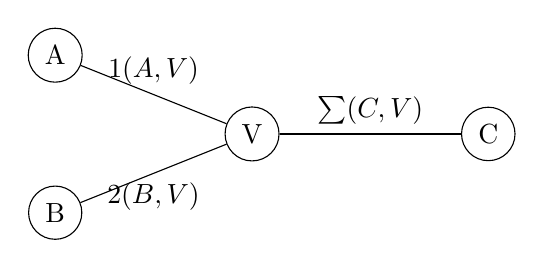
\begin{tikzpicture}
        % Nodi
        \node[circle, draw] (A) at (-0.5,1) {A};
        \node[circle, draw] (B) at (-0.5,-1) {B};
        \node[circle, draw] (V) at (2,0) {V};
        \node[circle, draw] (C) at (5,0) {C};

    
        % Archi
        \draw[-] (A) -- (V) node[midway, above] {$1(A,V)$}; % Arco da A a B
        \draw[-] (B) -- (V) node[midway, below] {$2(B,V)$}; % Arco da B a D
        \draw[-] (V) -- (C) node[midway, above] {$\sum(C,V)$}; % Arco da D a C

    
    \end{tikzpicture}
\end{center}
Risolvere un CSP significa:
\begin{itemize}
    \item Trovare uno \textbf{stato obiettivo}
    \item Dimostrare che è \textbf{insoddisfacibile}
\end{itemize}

\subsection{Tecniche per il CSP}
Dal momento che noi conosciamo apriori i vincoli del problema, tali informazioni ci permettono di fare potature
nell'grafo dei vincoli molto più efficaci, ossia riducendo i domini delle variabili, eliminando i valori che violano
i vincoli del problema; questa tecnica è detta \textbf{Constraint Propagation} e ve ne sono di 3 tipi:
\paragraph{Consistenza di Nodo.}Si applica ai \textbf{vincoli unari}: un nodo si dice consistente se il dominio non contiene valori
che violano un vincolo unario. Il concetto di consistenza di nodo permette di ridurre un dominio escludendo i valori
inammissibili.
\paragraph{Consistenza ad Arco.}Si applica ai \textbf{vincoli binari}: un nodo $X_i$ si dice \textit{consistente ad arco} a $X_j$
se per ogni valore in $D_i$ esiste almeno un valore in $D_j$ che soddisfa il vincolo binario. Grazie a questo concetto di consistenza,
è possibile escludere da un dominio tutti i valori che impediscono la consistenza ad arco con l'altra variabile.
Una cosa da mettere in evidenza è che un vincolo binario \textbf{deve essere letto in entrambe le direzioni}, per esempio,
$A > B$ deve essere letto sia come $A > B$ sia come $B < A$, in questa maniera possiamo togliere da $D_A$ tutti i valori
per cui non esiste alcun valore minore in $D_B$, così come posso escludere da $D_B$ tutti i valori che sono maggiori di ogni altro
elemento in $D_A$.

\paragraph{Caso Patologico:} 
\begin{center}
    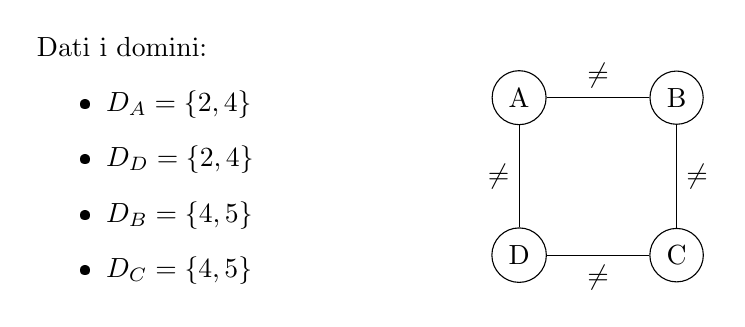
\begin{tikzpicture}
        % Posizioni dei vertici
        \node[circle, draw] (A) at (0, 2) {A};
        \node[circle, draw] (B) at (2, 2) {B};
        \node[circle, draw] (C) at (2, 0) {C};
        \node[circle, draw] (D) at (0, 0) {D};
        
        % Collegamenti tra i vertici
        \draw (A) -- (B) node[midway, above] {$\neq$};
        \draw (B) -- (C) node[midway, right] {$\neq$};
        \draw (C) -- (D) node[midway, below] {$\neq$};
        \draw (D) -- (A) node[midway, left] {$\neq$};
    
        \node[anchor=east] at (-3, 1.2) {
            \begin{minipage}{3cm}
                Dati i domini:
                \begin{itemize}
                    \item $D_A = \{2,4\}$
                    \item $D_D = \{2,4\}$
                    \item $D_B = \{4,5\}$
                    \item $D_C = \{4,5\}$
                \end{itemize}
            \end{minipage}
        };
    \end{tikzpicture}
\end{center}
In realtà l'intero grafo è già \textbf{Arc-Consistent}